%\documentclass[wcp,gray]{jmlr} % test grayscale version
\documentclass[10pt]{jmlr}% former name JMLR W\&CP
%\documentclass[pmlr]{jmlr}% new name PMLR (Proceedings of Machine Learning)

 % The following packages will be automatically loaded:
 % amsmath, amssymb, natbib, graphicx, url, algorithm2e
 \usepackage{amsmath,amssymb,graphicx,url}
 \graphicspath{ {./Figures/} }

 %\usepackage{rotating}% for sideways figures and tables
\usepackage{longtable}% for long tables

 % The booktabs package is used by this sample document
 % (it provides \toprule, \midrule and \bottomrule).
 % Remove the next line if you don't require it.
\usepackage{booktabs}
 % The siunitx package is used by this sample document
 % to align numbers in a column by their decimal point.
 % Remove the next line if you don't require it.
\usepackage[load-configurations=version-1]{siunitx} % newer version
 %\usepackage{siunitx}

% Package to make table with multi rows and columns
\usepackage{multirow}
 
 % to do
\usepackage{xcolor}
\newcommand\todo[1]{\textcolor{red}{#1}}

 % change the arguments, as appropriate, in the following:
\jmlrvolume{}
\jmlryear{}
\jmlrworkshop{STA723 -- Case Study 1}
\jmlrproceedings{}{}


\usepackage[toc,page]{appendix}

\usepackage{geometry}
\geometry{letterpaper, margin=0.9in}



% start article
% \titlebreak
% \footnote{}
% \textsf

\title[Modeling Price and Popularity of AirBnB listings in New-York]{Modeling Price and Popularity of AirBnB listings in New-York}	%\titletag{\thanks{XXX}} % leave empty?

 % Use \Name{Author Name} to specify the name.
 % If the surname contains spaces, enclose the surname
 % in braces, e.g. \Name{John {Smith Jones}} similarly
 % if the name has a "von" part, e.g \Name{Jane {de Winter}}.
 % If the first letter in the forenames is a diacritic
 % enclose the diacritic in braces, e.g. \Name{{\'E}louise Smith}

 % Authors with different addresses:
 
 \author[Jiang, Morsomme, Nwankwo]{Melody Jiang \and Raphael Morsomme \and Ezinne Nwankwo}
 \date{\today} % Date, can be changed to a custom date

 % Three or more authors with the same address:
 % \author{\Name{Author Name1} \Email{an1@sample.com}\\
 %  \Name{Author Name2} \Email{an2@sample.com}\\
 %  \Name{Author Name3} \Email{an3@sample.com}\\
 %  \addr Address}

 % Authors with different addresses:
 % \author{\Name{Author Name1} \Email{abc@sample.com}\\
 % \addr Address 1
 % \AND
 % \Name{Author Name2} \Email{xyz@sample.com}\\
 % \addr Address 2
 %}

% leave editor's section empty?
%\editor{Editor's name}
% \editors{List of editors' names}

\begin{document}

\maketitle

\begin{abstract}
In this paper, we seek to understand factors about a typical Airbnb listing that influence its price and popularity. We analyze a dataset with a total of 48,895 Airbnb listings in New York and 16 variables. We focus on feature engineering and fit two types of models: linear model using Bayesian Model Averaging and random forest with popularity and price as the outcome variables. Ultimately, our main finding in which all of our models agreed with was that room type and borough play a huge role in determining price and popularity. 
\end{abstract}

%%%%%%%%%%%%%%%%%%%%%%%%%%%%%%%%%%%%%%%%%%%%%%%%%%%%%%%%%%%%%
% INTRODUCTION
%%%%%%%%%%%%%%%%%%%%%%%%%%%%%%%%%%%%%%%%%%%%%%%%%%%%%%%%%%%%%
\section{Introduction}
\label{sec:intro}

Airbnb has quickly grown into one of the largest online marketplace for arranging long or short term stays at homes and appartments owned by people. Airbnb does not own any of the property on its site; instead it acts as a broker between customers and hosts and earns a commission from each booking. Hosts have full control over aspects such as pricing, how to advertise their listings, and how often their listing is available throughout the year. For this project, we are interested in modelling price and popularity of listsings in order to best advise hosts on tactics that will maximize their profit and popularity on the platform. This includes (i.) identifying influential factors on the price and popularity of the listing (ii.) identifying heterogeniety across boroughs and neighborhoods, in particular which ones have the heaviest traffic and highest prices (iii.) identifying hetoergeneity across listing type and (iv.) providing recommendations on listing location and names. 


%%%%%%%%%%%%%%%%%%%%%%%%%%%%%%%%%%%%%%%%%%%%%%%%%%%%%%%%%%%%%
% METHODS
%%%%%%%%%%%%%%%%%%%%%%%%%%%%%%%%%%%%%%%%%%%%%%%%%%%%%%%%%%%%%
\section{Methods}
\label{sec:method}

\subsection{Data Preparation}
\label{sec:data}
The quality of the data is questionable and the meaning of some variables is unclear. For instance, the data set contains listings with a price superior to USD$5,000$ per night or equal to $0$, a minimum number of nights superior to $1,000$ and an average number of monthly review superior to $50$. It was also unclear what the price variable represents - average price of booking, average listed price or current listed price? We also did not know how the variable availability\_365 was constructed - average number of available days per year, number of available days in the last year, or current number of available days.

For these reasons, we decide to clean the dataset by removing listings that are not typical of the Airbnb platform. That is, we remove listing for long-term stays and listings that are owned by businesses (some owners possess several dozens of listings), since we believe that the set of factors determining their price and popularity strongly differs from that of a typical \textit{short-term}, \textit{privately owned} Airbnb listing. We also exclude listings that have not been reviewed in the last $12$ months since factors that mattered several years ago may no longer be relevant. The resulting data set contains $24,255$ \textit{short-term}, \textit{active} and \textit{privately owned} listings.

\subsection{Feature Engineering}
\label{sec:feature}
\subsubsection{Spatial Variables}
\figureref{fig:map_eda} suggests that the most expensive listings are located close to metro stations. We therefore construct a variable indicating the proximity of the closest metro station. The proximity between two locations $x$ and $y$ is computed with
$\text{proximity}(x,y) = \dfrac{1}{\text{dist}(x,y)}$
where $\text{dist}(x,y)$ measures the distance between $x$ and $y$. We use the \textit{manhattan} distance
$$\text{dist}_{\text{Manhattan}}(x,y) = |lat_x - lat_y| + |long_x - long_y|$$
which approximates the distance traveled by a pedestrian walking on the perpendicular streets of New-York.

Similarly, we compute the average proximity to the $36$ attractions with
$$\text{proximity}_\text{attraction}(x) = \dfrac{1}{36} \sum_{i=1}^{36} \dfrac{1}{\text{dist}_{\text{Manhattan}}(x,\text{attraction}_i)}$$

\subsubsection{Textual Variables}
First, we conducted a sentiment analysis on the listing names in order to construct a variable indicating the sentiment of the listing name, that is, how positive the name sounds. The sentiment of a document $W = (w_1, w_2, \dots, w_n)$ composed of $n$ words is
$$\text{sentiment}(W) = \dfrac{1}{n} \sum_{i=1}^{n} \text{dictionary}(w_i)$$
where $\text{dictionary}(w_i)$ indicates the sentiment of the word $w_i$ according to some sentiment dictionary. Since the listing names are relatively short, we use the Affin dictionary which provides a gradual sentiment metric ranging from $-5, 5$; the other existing sentiment dictionaries only provide a binary metric ($-1$, $1$) and would provide a sentiment that is too coarse for such short documents.

In addition, we attempted to model the origin of the owner's name. The rationale for this is that we expect renters to be less likely to book a listing whose owner has a name that does not look familiar. We obtained the relatively frequency of a someone's name in the data as a measurement of how common the name is. Since some owners own multiple listings, we filter by unique ID before computing the frequencies.



\subsection{Model}
We implemented two models, Bayesian Model Averaging (BMA) in linear models and random forests (RF). For BMA, we build two models separately for log price and log popularity using all the variables as a linear combination of predictors. We exclude latitude and longitude because there is no inpretable relationship between the magnitiude of, say, latitude and outcome variables. After sensitivity analysis, we decided to use a Cauchy prior for the predictors and a uniform prior over the model space, which assigns equal probability to all the models. We use an MCMC algorithm with $10^{16}$ iterations to sample from the model space of $2^{15}$ models. Lastly, we approximate the marginal inclusion probabilities of the predictors by taking the p-values from p simple linear regressions. The posterior inclusion probabilities (PIP) of each predictor was primarily what we used to determine influential factors in price and popularity of a listing. 

For the RF models, we used all the predictors including longitude and latitude since this class of models does not make any linearity assumptions between predictors and outcome variable. We build these models using 1900 trees each built on subsamples of 19000 data points. Due to computational challenges, we could not go beyond this number of trees and subsamples. For the split criteria, we randomly sampled $m = \frac{p}{3} = 4$ variables as candidates for the split (Note that this is the default value for regression) and $n_{leaf} \geq 5$. We used a variable importance measure that is based on an increase in node purity, or Gini-based importance. It is is calculated based on the reduction in sum of squared errors whenever a variable is chosen to split.

After our initial explanatory analysis, there was only a slight suggestion of linearity for some of the predictors. This provides further justification for our choice to fit a linear and non-linear model and compare the results.


%%%%%%%%%%%%%%%%%%%%%%%%%%%%%%%%%%%%%%%%%%%%%%%%%%%%%%%%%%%%%
% RESULTS
%%%%%%%%%%%%%%%%%%%%%%%%%%%%%%%%%%%%%%%%%%%%%%%%%%%%%%%%%%%%%
\section{Results}
\label{sec:results}

%%%%%%%%%%%%%%%%%%%%%%%%%%%%%%%%% EDA
\subsection{EDA}

\figureref{fig:length_stay_density} shows the distribution of required minimum number of nights to book a listing. We observe that minimum number of nights is concetnrated at below 14 days and around 30 days. \figureref{fig:availability_density} displays the distribution of days that listings are available for booking in a year. We see that there are data concentrated at 0, which means these listings are not open for booking. Such observation would inform our data cleaning.

To address the quesstion of whether the type of listing (shared room, private room, entire home) vary across boroughs, we performed a chi-square test and plotted the results in \figureref{fig:room_type}. The p-value of the chi-square test was less than $10^{-16}$. In \figureref{fig:room_type}, the size of dots represents the absolute standardized residuals. The color represents the value of standardized residuals. We see that difference in room types is most pronounced in Manhattan and Queens. Manhattan has more entire home than expected and Queens has more private room than expected.

\figureref{fig:map_eda} shows a spatial map of  of listings, metro stations, and attractions. Black dots represent metro stations, gree dots attractions, blue dots listings priced at bottom 80\%, and red dots are listings priced at top 20\%. We observe that listings priced at top 20\% distribute close to metro stations. This observation motivates us to include spatial in formation of metro stations as explanatory variables.



%%%%%%%%%%%%%%%%%%%%%%%%%%%%%%%%% MAIN FINDINGS
\subsection{Main Findings}

From our models, we were able to identify the top influential factors for price and popularity. For price, the BMA and RF models agree that room type and boroughs are very influential factors. BMA flagged the variable "name host special" as being significant with the highest value for the estimated effect on price being a 10.42 increase in the average log price given that the name of the host was not common while holding all other variables in the model constant. The next largest estimate was "Room type:Entire Home/Apt", which had a 0.74 change in the average log price given that the room type was an entire home or apartment while holding other variables in the model constant. Next, we saw that the models agreed that neighborhood group, minimum nights and listing sentiments are very influential factors in determining the popularity of a listing. In BMA model, the significant predictors were "listing count", "minimum nights", "name listing length", "number of reviews", and "listing sentiment". The variable "listing sentiment" had the largest estimate effect on log popularity with a 0.16 decrease in the average log popularity holding all other variables in the model constant. 

Appendix B contains outputs from each model, with the predictors ordered from most influential to least influential using posterior inclusion probabilities from the BMA models and variable importance from the RF models. The tables also include the estimated effects for the other variables in the model, a majority of which had an estimated effect of zero. 

%%%%%%%%%%%%%%%%%%%%%%%%%%%%%%%%% SENSITIVITY ANALYSIS
\subsection{Model Checking and Sensitivity Analysis}

Our model was very sensitive to outliers. When we first fit our models, we noticed some outliers in the residuals plot, and thus decided to remove points that were three times the standard deviation away from the mean of the outcome. After refitting, the model residual plots looked much better and had better $R^2$ values, as shown in \figureref{fig:price_diag} and \figureref{fig:pop_diag}. For the BMA models, we also varied the choice in prior by testing out the g-prior for g = 1, 5, 8, 50, 100, 500, 1000. The results did not change for the different priors. Lastly, for the RF models, we varied m and the minimum $n_{leaf}$. The final values that we used for those parameters did not result in a change in MSE. 

\section{Discussion}
\label{sec:conclusion}

(i) As shwon in our main findings, the most influential factors on price that BMA and RF agree on are room type and borough. For popularity, influential factors that both models agree on are minimum nights, listing sentiment, and borough. (iii) As shown in the EDA section, the type of listing does vary across neighbourhoods, since the p-value indicates significance. We have also seen the most pronounced difference in Mahhattan and Queens, where Manhattan has more entire home than expected and Queens has more private room than expected. (ii)(iv) Yes, there is heterogeneity across boroughs, and Manhattan is the most pricy. To make our listing the most pricy, We would locate an entire home/apartment in Manhattan and use a common name as host. Whether to use positive words in the name of listing does not affect the price.

We have seen in Results section that variable importance of BMA and random forest do not agree completely. This could be due to nonlinear trend that is hard to pick up in EDA. We could investigate this issue further in future work.

Regarding BMA for popularity, we have seen the anti-intuitive result that popularity declines as sentiment of listing name becomes positive. This calls for a more detailed analysis of listing names.

For future improvements, we would like to include spatial modeling. For example, we could model spatial relationship between houses, as \cite{james2005apartment} has shown that OLS including just boroughs as spatial information does not work well . In addition, we could utilize domain-specific knowledge to improve our modeling of price. We could potentially use a finite mixture model to identify submarkets as in the study by \cite{belasco2012using}. We could also draw from knowledge in marketing to improve our feature engineering, for example consider pricing as an explanatory variable for popularity.





%%%%%%%%%%%%%%%%%%%%%%%%%%%%%%%%%%%%%%%%%%%%%%%%%%%%%%%%%%%%%
% APPENDIX
%%%%%%%%%%%%%%%%%%%%%%%%%%%%%%%%%%%%%%%%%%%%%%%%%%%%%%%%%%%%%
\newpage
\appendix

%%%%%%%%%%%%%%%%%%%%%%%%%%%%%%%%% BOX COX
\section{Figures}
\label{appendix:fig}

\begin{figure}[htbp]
	\centering
	\caption{Distribution of minimum number of nights.}
	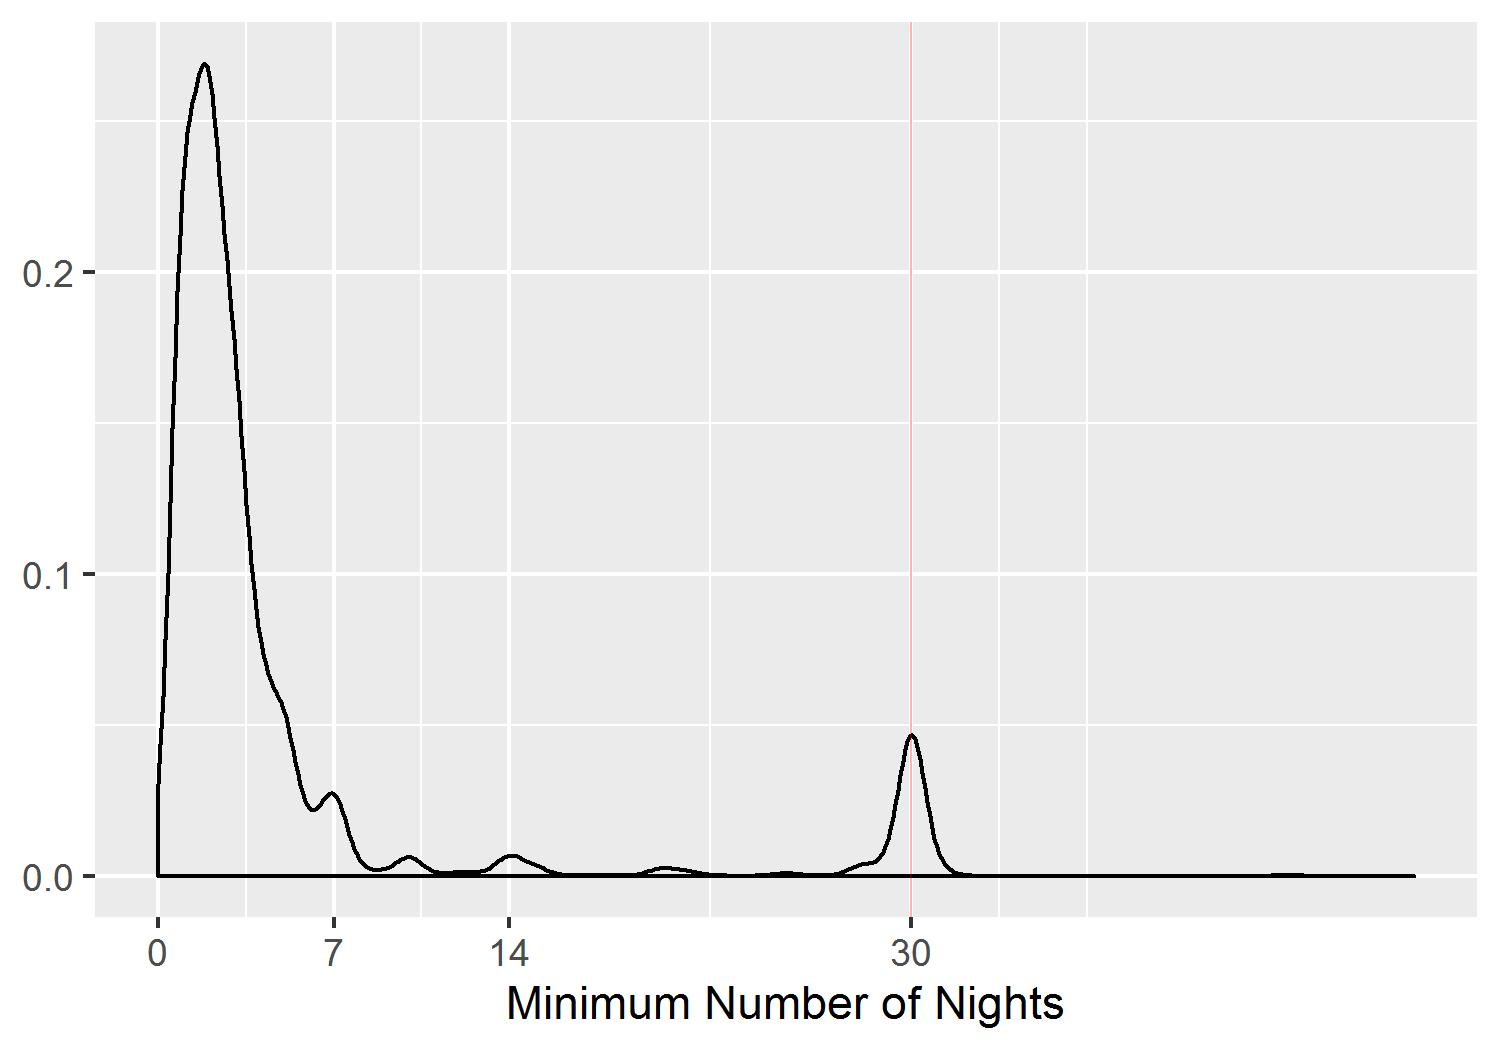
\includegraphics[width=0.5\linewidth]{length_stay_density.jpeg}
	\label{fig:length_stay_density}
\end{figure}

\begin{figure}[htbp]
	\centering
	\caption{Distribution of number of days available for booking.}
	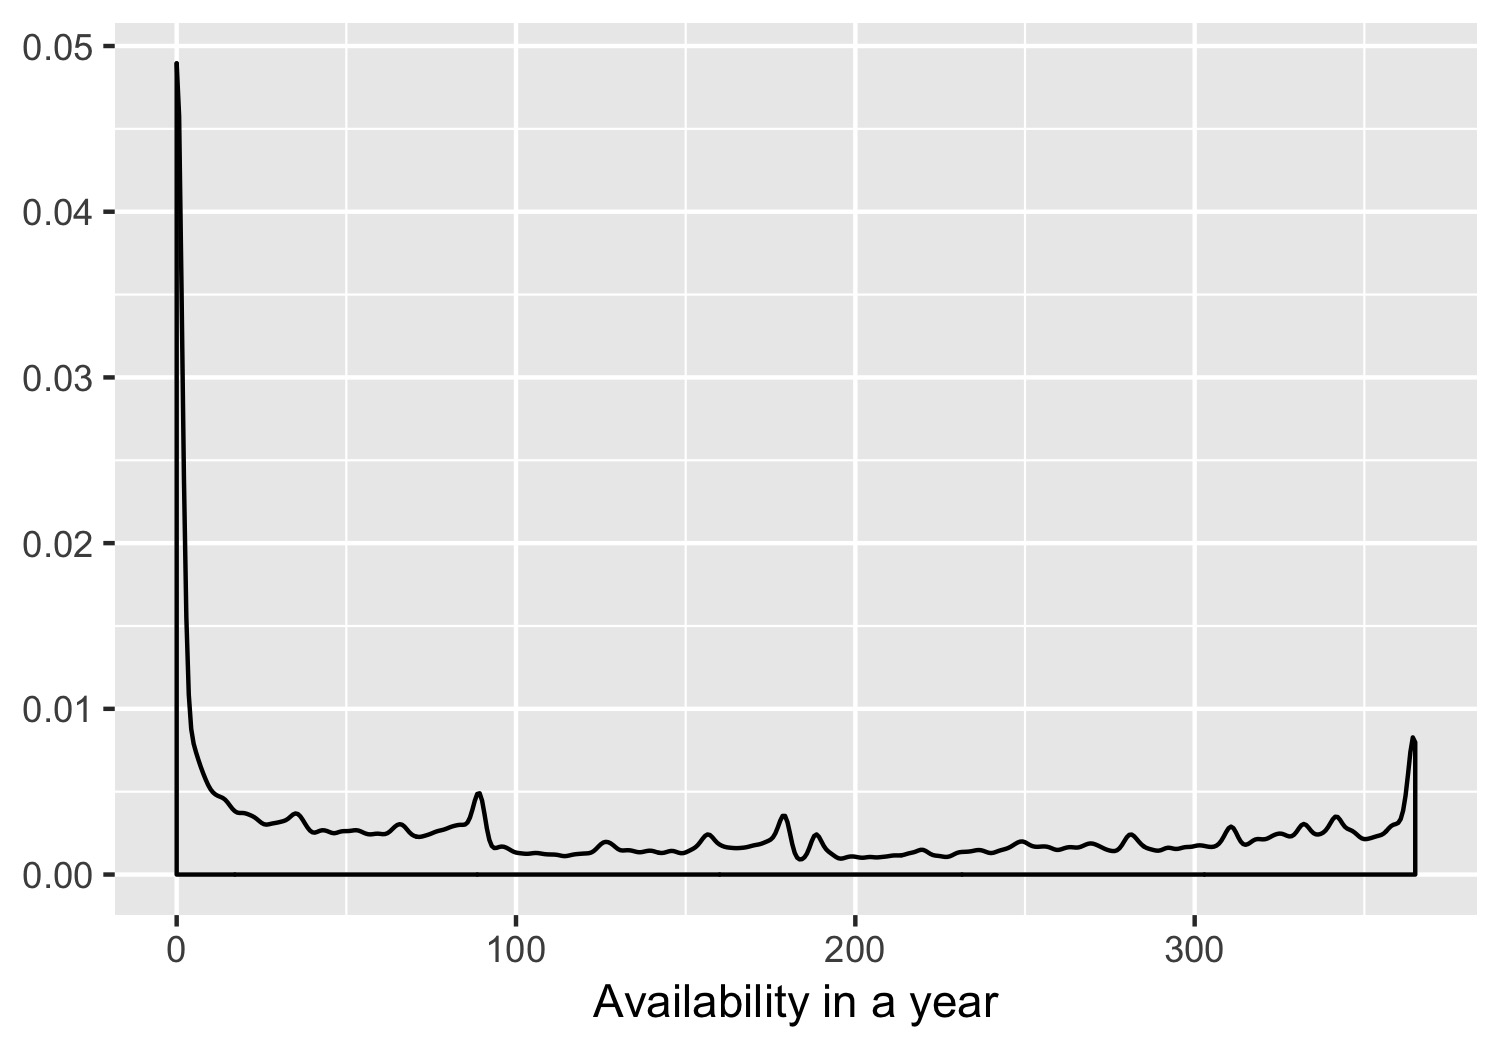
\includegraphics[width=0.5\linewidth]{availability_density.jpeg}
	\label{fig:availability_density}
\end{figure}

\begin{figure}[htbp]
	\centering
	\caption{Output from chi-squared test.}
	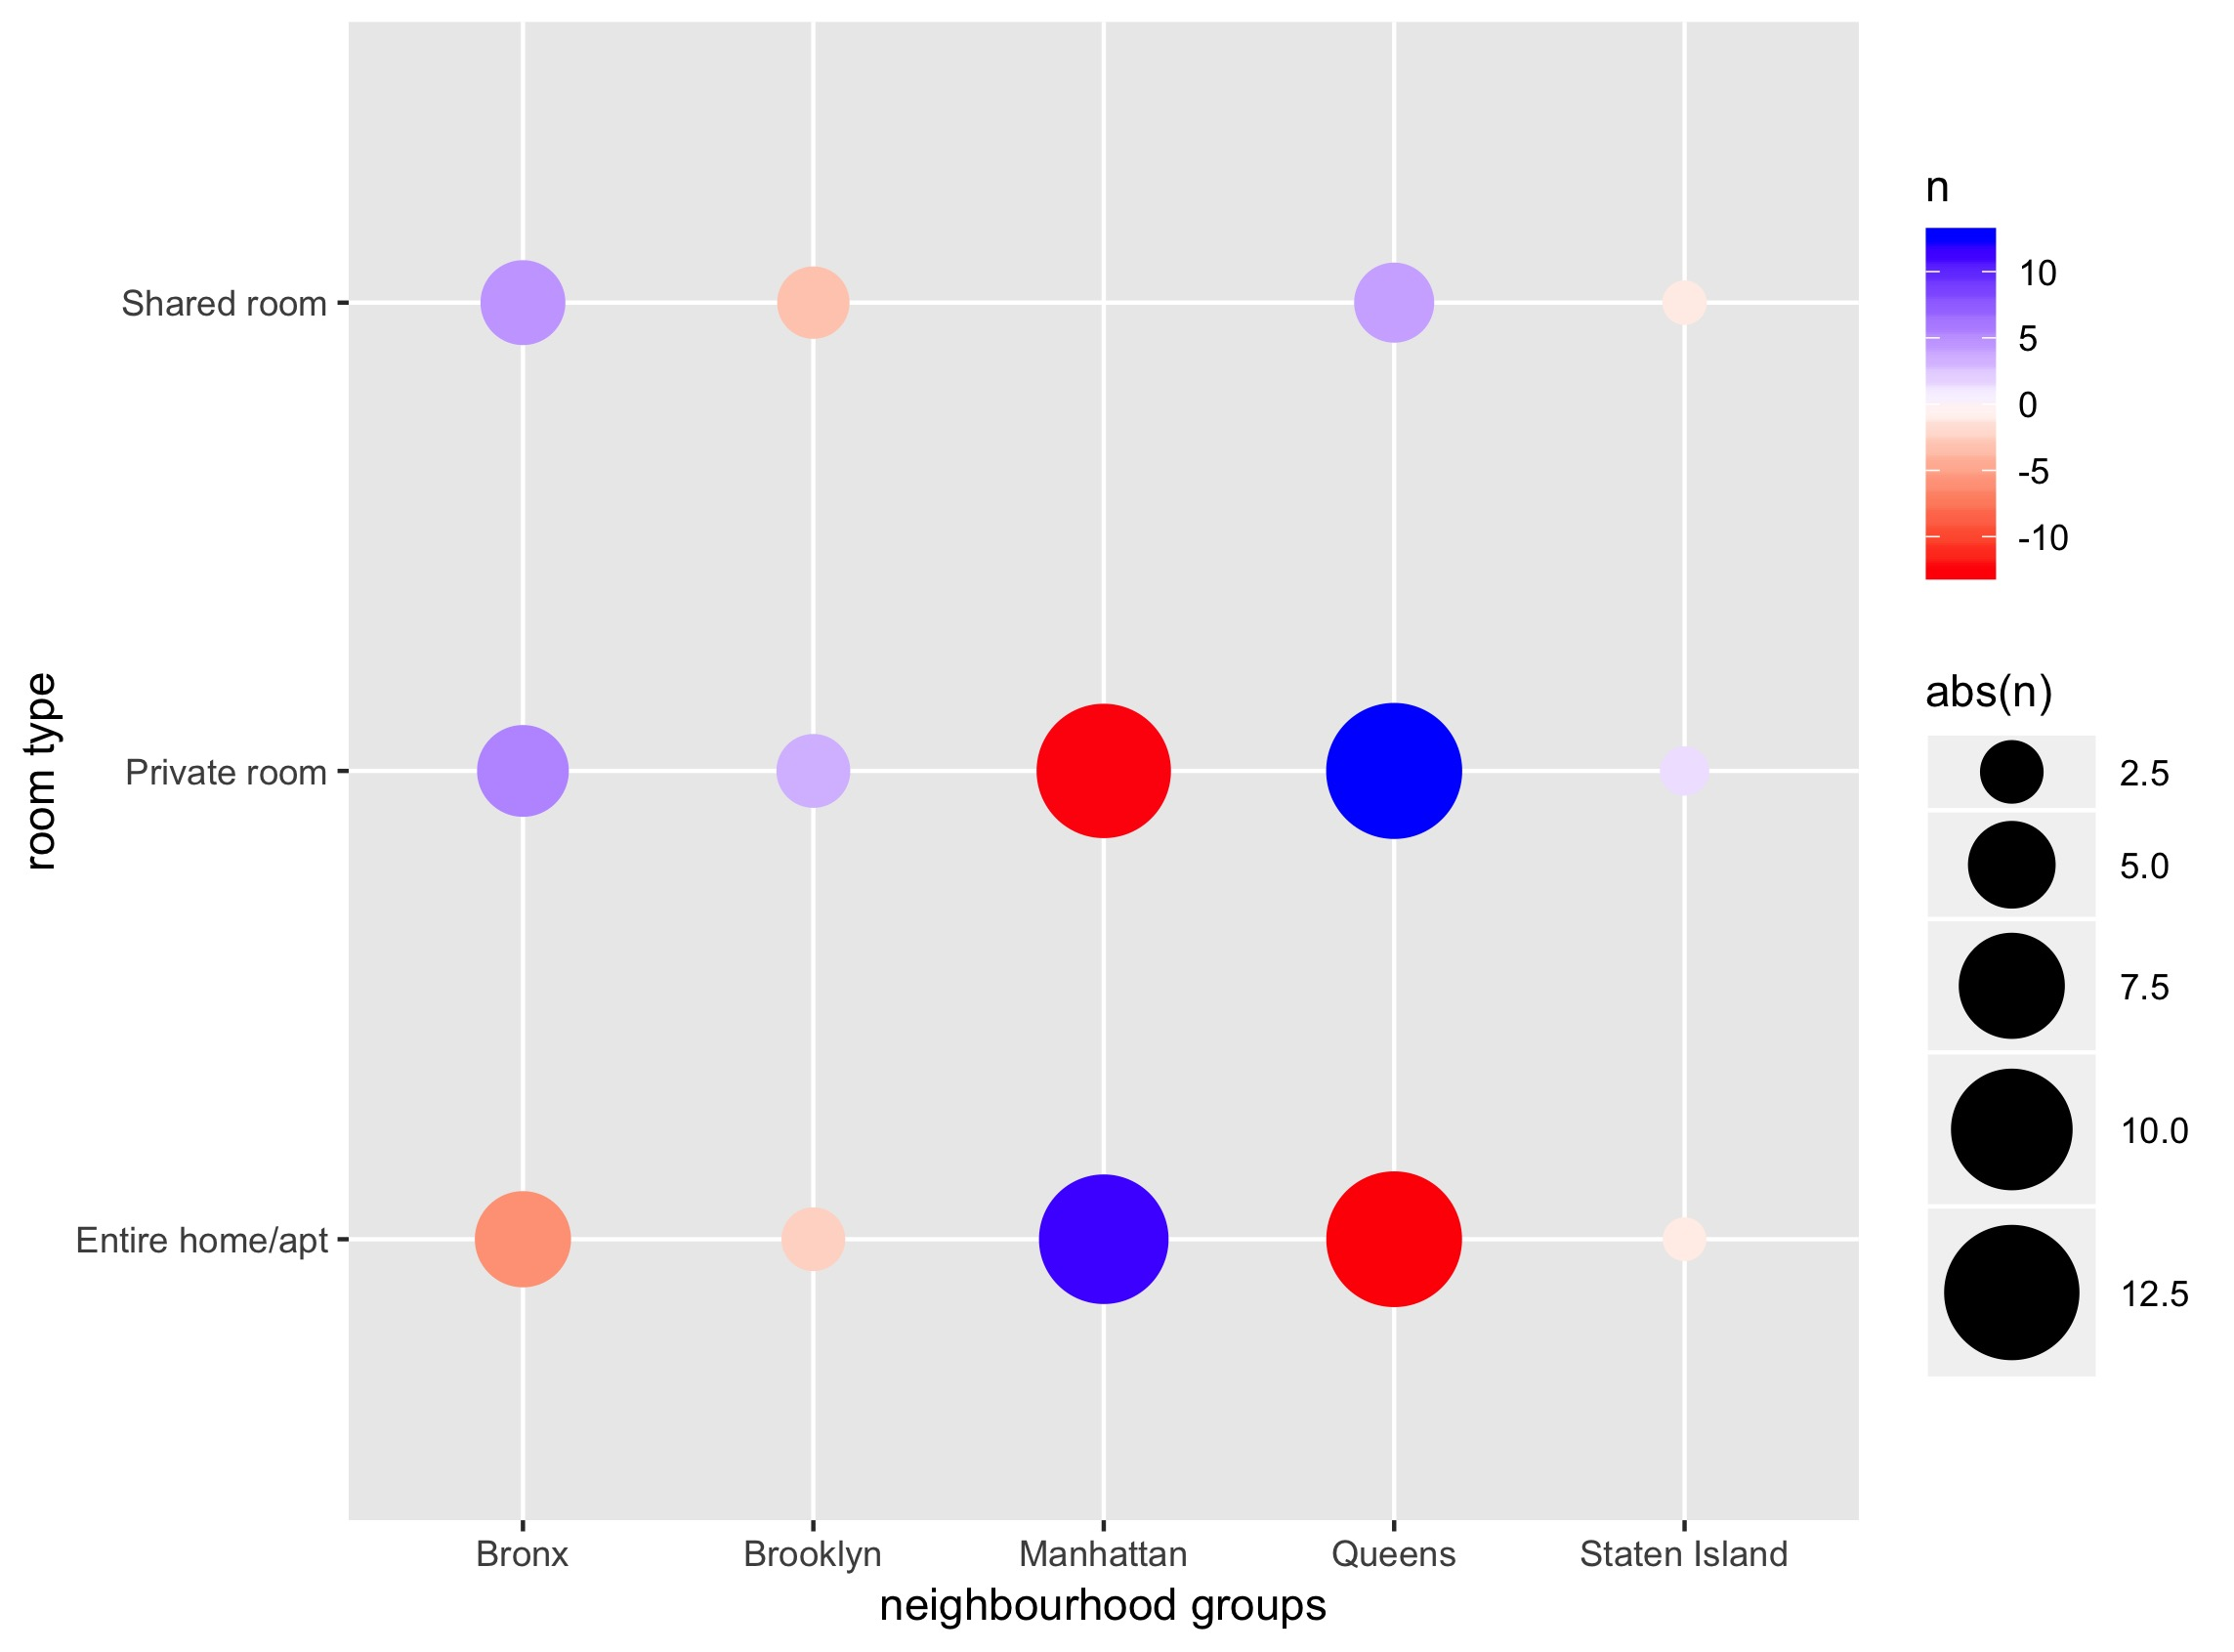
\includegraphics[width=0.5\linewidth]{room_type.jpeg}
	\label{fig:room_type}
\end{figure}

\begin{figure}[htbp]
	\centering
	\caption{Map of listings, metro stations, and attractions. Black dots are metro stations, gree dots are attractions, blue dots are listings priced at bottom 80\%, and red dots are listings priced at top 20\%}
	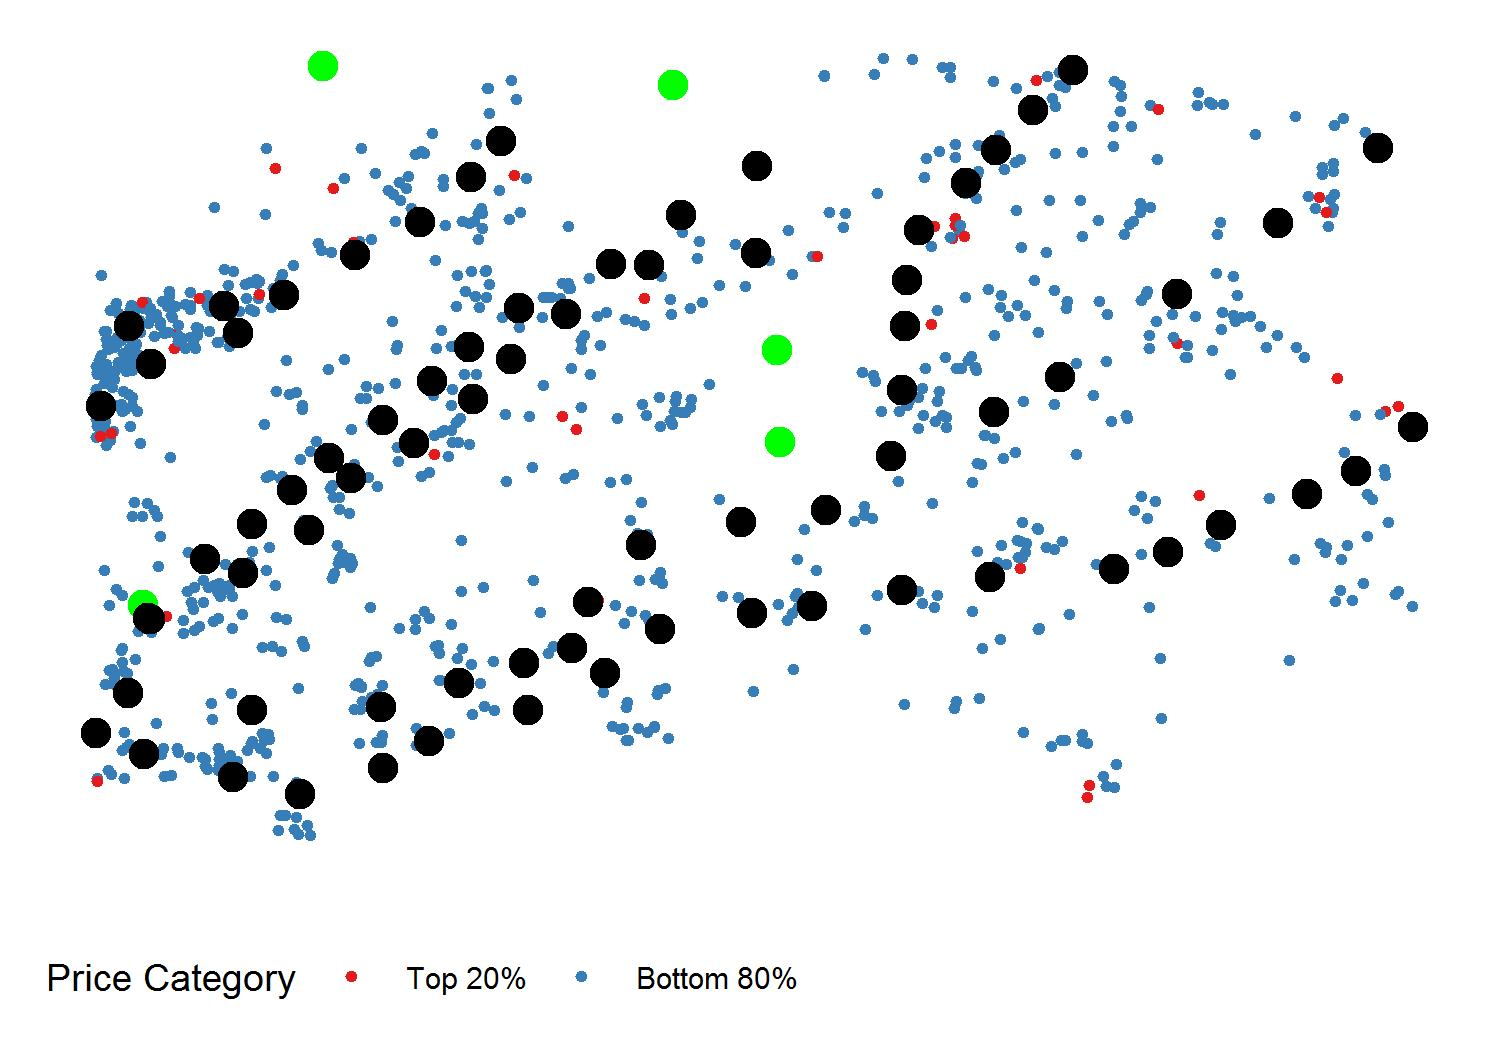
\includegraphics[width=0.5\linewidth]{map_eda.jpeg}
	\label{fig:map_eda}
\end{figure}

\begin{figure}[htbp]
	\centering
	\caption{Model diagnostics for BMA for price}
	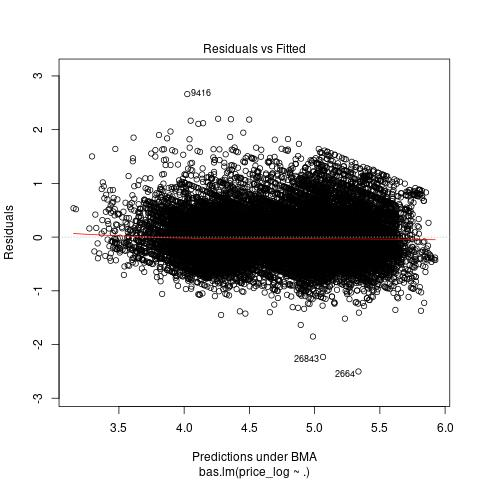
\includegraphics[width=0.5\linewidth]{price_diagnostic_plot.jpeg}
	\label{fig:price_diag}
\end{figure}

\begin{figure}[htbp]
	\centering
	\caption{Model diagnostics for BMA for popularity}
	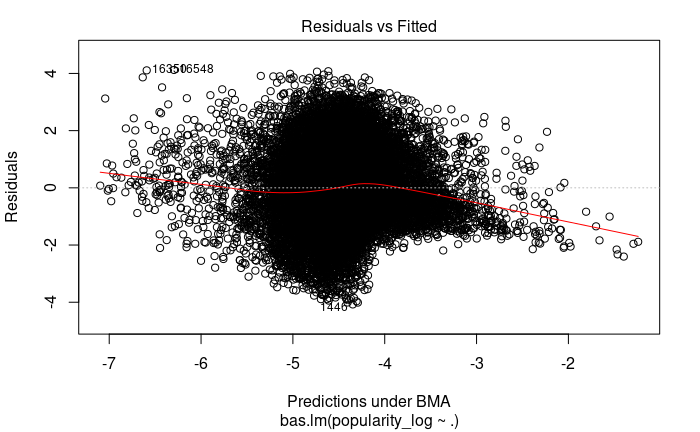
\includegraphics[width=0.5\linewidth]{pop_diagnostic_plot.png}
	\label{fig:pop_diag}
\end{figure}

\begin{figure}[htbp]
	\centering
	\caption{Residuals for price BMA model}
	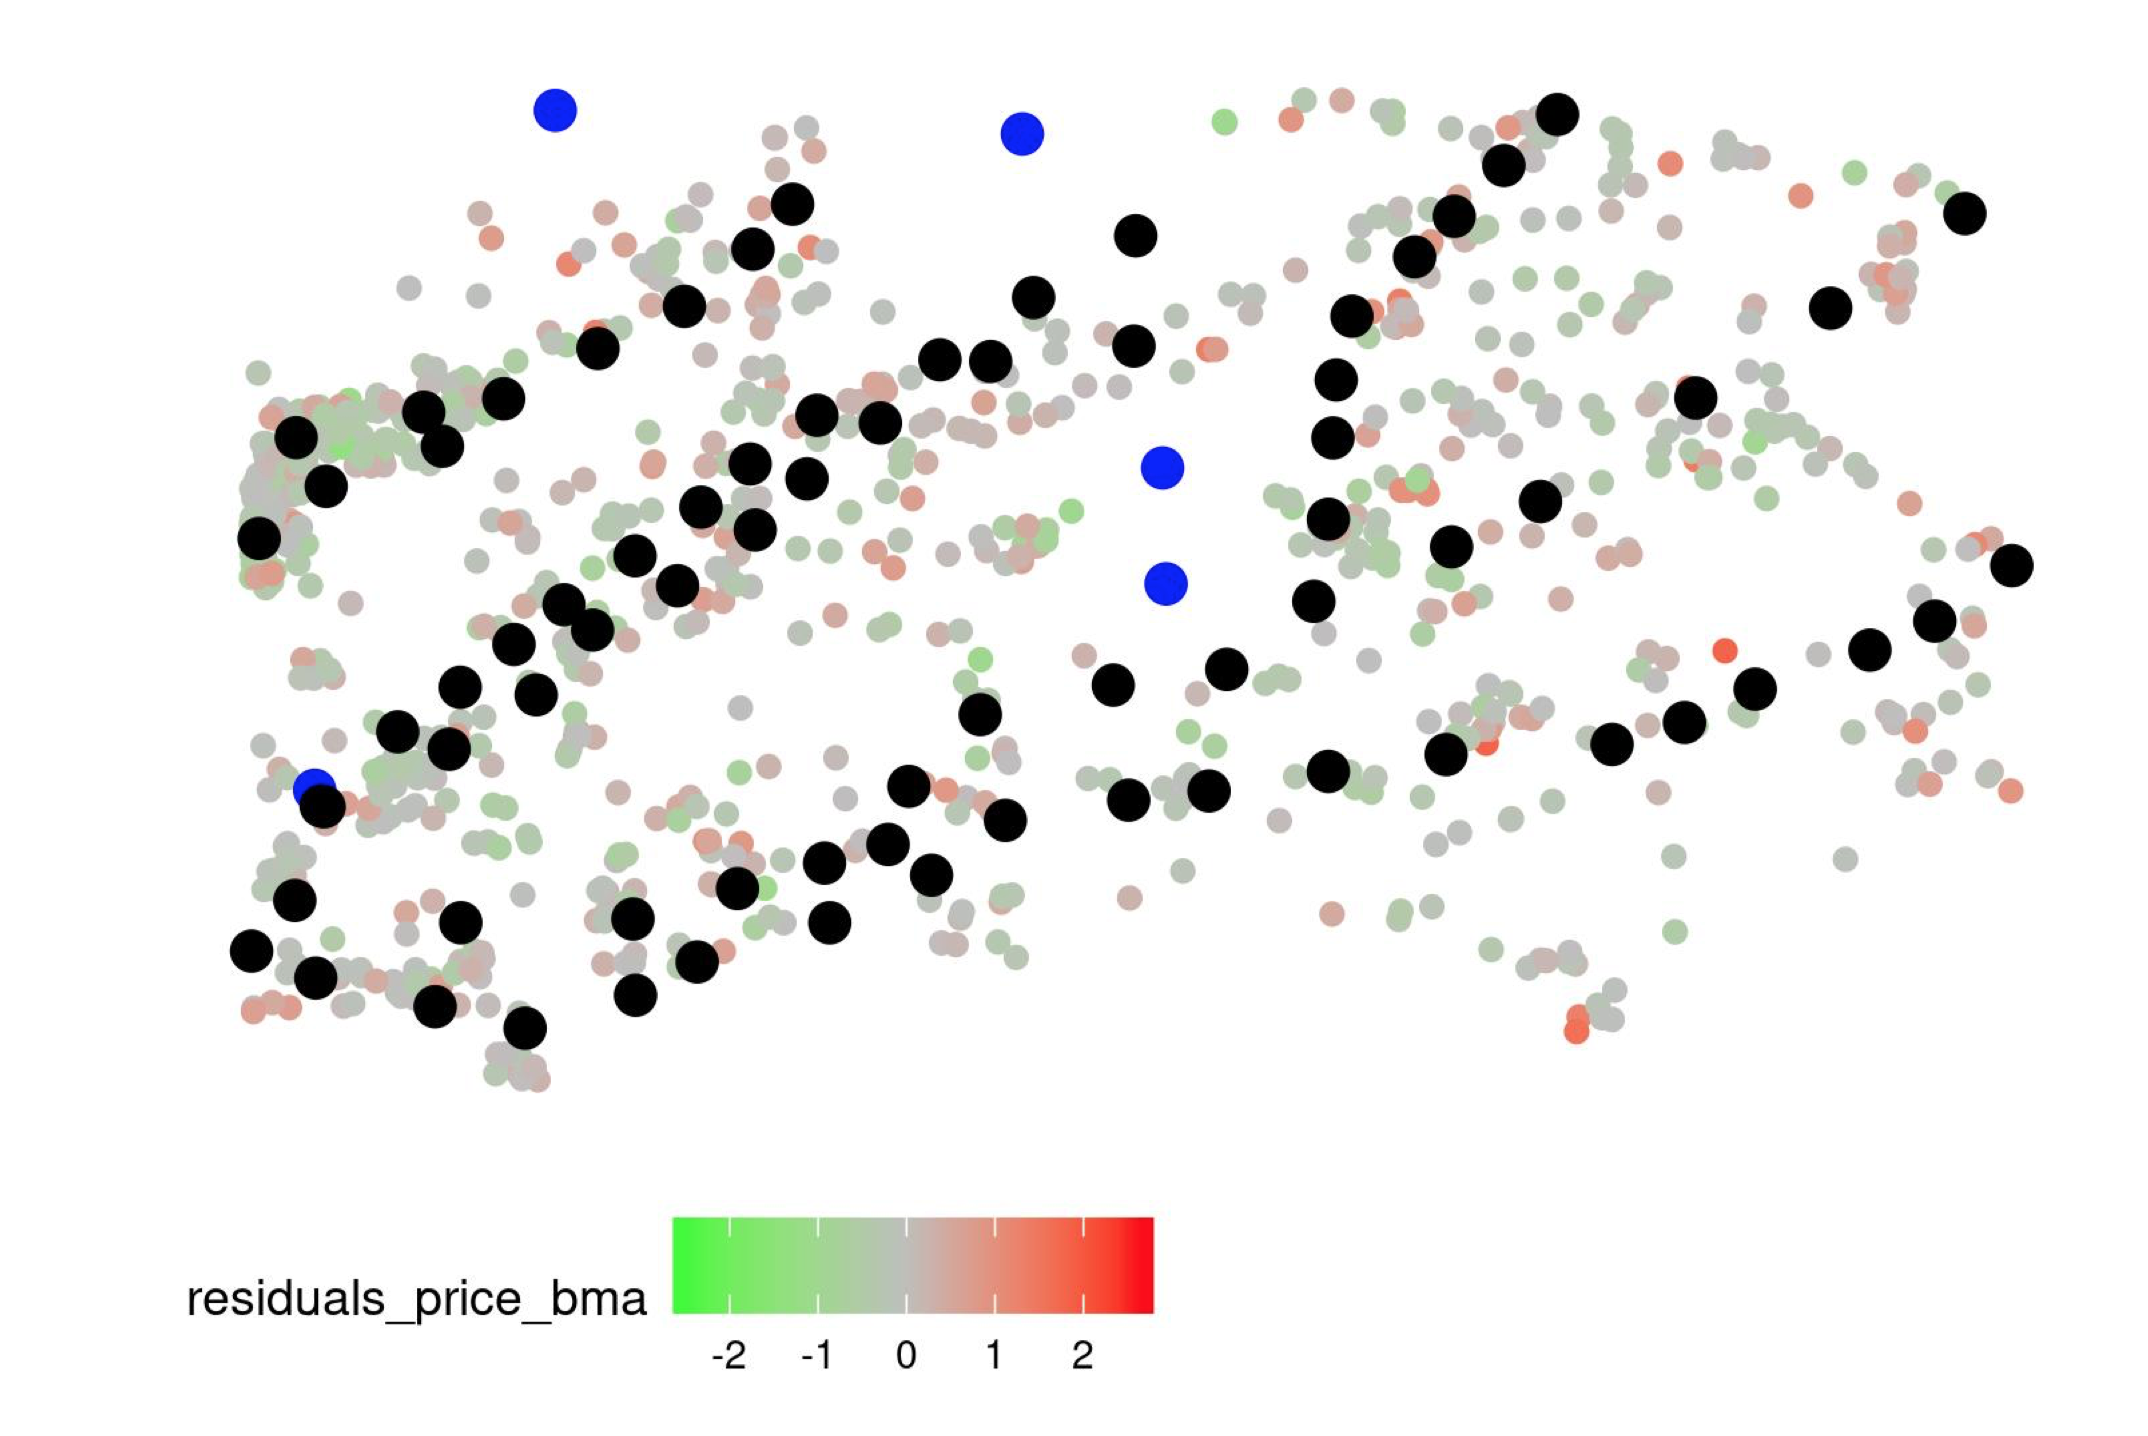
\includegraphics[width=0.5\linewidth]{residual_map_price.png}
	\label{fig:map_residuals}
\end{figure}


\newpage  % ensures that all figures remain together in appendix B

%%%%%%%%%%%%%%%%%%%%%%%%%%%%%%%%% MODEL CHECKING

\section{Full Model Output}

% latex table generated in R 3.6.1 by xtable 1.8-4 package
% Mon Feb  3 21:05:30 2020
\begin{table}[ht]
\centering
\begin{tabular}{rlr}
  \hline
 & Predictors & Variable.Importance \\ 
  \hline
1 & last\_review & 978.10 \\ 
  2 & name\_listing\_sentiment & 107.88 \\ 
  3 & name\_host\_freq & 101.15 \\ 
  4 & availability\_365 & 100.73 \\ 
  5 & Room\_type & 95.16 \\ 
  6 & number of reviews & 94.24 \\ 
  7 & reviews\_per\_month & 90.71 \\ 
  8 & proximity\_metro & 89.26 \\ 
  9 & calculated\_host\_listings\_count & 88.53 \\ 
  10 & Neighbourhood\_group & 61.00 \\ 
  11 & type\_stay & 53.69 \\ 
  12 & name\_host\_special & 47.78 \\ 
  13 & name\_listing\_length & 39.16 \\ 
  14 & proximity\_attraction & 16.42 \\ 
   \hline
\end{tabular}
\end{table}


% latex table generated in R 3.6.1 by xtable 1.8-4 package
% Mon Feb  3 21:49:38 2020
\begin{table}[ht]
\centering
\begin{tabular}{rlr}
  \hline
 & Predictors & Variable.Importance \\ 
  \hline
1 & number\_of\_reviews & 199.74 \\ 
  2 & latitude & 62.77 \\ 
  3 & listing\_sentiment & 59.50 \\ 
  4 & minimum\_nights & 57.85 \\ 
  5 & neighbourhood\_group & 54.93 \\ 
  6 & room\_type & 50.03 \\ 
  7 & reviews\_per\_month & 49.69 \\ 
  8 & longitude & 45.87 \\ 
  9 & name\_listing\_length & 41.50 \\ 
  10 & name\_host\_special & 35.34 \\ 
  11 & popularity\_log & 33.77 \\ 
  12 & proximity\_attraction & 20.73 \\ 
  13 & listing\_count & 8.76 \\ 
  14 & name\_host\_freq & 8.72 \\ 
  15 & proximity\_metro & 0.42 \\ 
   \hline
\end{tabular}
\end{table}


\begin{table}[ht]
\centering
\begin{tabular}{rlrrrrl}
  \hline
 & Predictors & PIP & Estimate & Lower.Confint & Upper.Confint & Significance \\ 
  \hline
1 & Intercept & 1.00 & 4.70 & 4.70 & 4.71 & * \\ 
  2 & name\_host\_freq & 1.00 & 0.07 & 0.07 & 0.07 & * \\ 
  3 & Neighbourhood\_group:Manhattan & 1.00 & 0.17 & 0.15 & 0.18 & * \\ 
  4 & number of reviews & 1.00 & -0.01 & -0.02 & -0.01 & * \\ 
  5 & Room\_type:Entire home/apt & 1.00 & 0.74 & 0.73 & 0.75 & * \\ 
  6 & availability\_365 & 1.00 & 0.00 & 0.00 & 0.00 &  \\ 
  7 & name\_listing\_sentiment & 1.00 & 0.00 & 0.00 & 0.00 &  \\ 
  8 & last\_review & 1.00 & -0.00 & -0.00 & -0.00 &  \\ 
  9 & Neighbourhood\_group:Queens & 1.00 & -0.11 & -0.13 & -0.10 & * \\ 
  10 & name\_host\_special:True & 1.00 & 10.42 & 7.16 & 13.66 & * \\ 
  11 & Room\_type:Shared room & 1.00 & -0.51 & -0.54 & -0.47 & * \\ 
  12 & calculated\_host\_listings\_count & 1.00 & -0.01 & -0.02 & -0.01 & * \\ 
  13 & type\_stay:Long & 1.00 & 0.00 & 0.00 & 0.00 &  \\ 
  14 & Neighbourhood\_group:Bronx & 1.00 & -0.17 & -0.20 & -0.14 & * \\ 
  15 & name\_listing\_length & 1.00 & 0.06 & 0.04 & 0.08 & * \\ 
  16 & proximity\_metro & 0.89 & -0.00 & -0.00 & 0.00 &  \\ 
  17 & proximity\_attraction & 0.50 & -0.01 & -0.04 & 0.00 &  \\ 
  18 & reviews\_per\_month & 0.07 & -0.00 & -0.00 & 0.00 &  \\ 
  19 & Neighbourhood\_group:Staten Island & 0.02 & -0.00 & 0.00 & 0.00 &  \\ 
   \hline
\end{tabular}
\caption{Coeffients and 95\% Confidence Intervals from Price BMA model} 
\end{table}

% latex table generated in R 3.6.1 by xtable 1.8-4 package
% Mon Feb  3 21:53:10 2020
\begin{table}[ht]
\centering
\begin{tabular}{rlrrrl}
  \hline
 & Predictors & Estimate & Lower.Confint & Upper.Confint & Signifance \\ 
  \hline
1 & Intercept & 4.70 & 4.70 & 4.71 & * \\ 
  2 & Neighbourhood\_group:Manhattan & 0.17 & 0.15 & 0.18 & * \\ 
  3 & Neighbourhood\_group:Queens & -0.11 & -0.13 & -0.10 & * \\ 
  4 & Neighbourhood\_group:Staten Island & -0.00 & 0.00 & 0.00 &  \\ 
  5 & Neighbourhood\_group:Bronx & -0.17 & -0.20 & -0.14 & * \\ 
  6 & Room\_type:Entire home/apt & 0.74 & 0.73 & 0.75 & * \\ 
  7 & Room\_type:Shared room & -0.51 & -0.54 & -0.47 & * \\ 
  8 & number of reviews & -0.01 & -0.02 & -0.01 & * \\ 
  9 & last\_review & -0.00 & -0.00 & -0.00 & * \\ 
  10 & reviews\_per\_month & -0.00 & -0.00 & 0.00 &  \\ 
  11 & calculated\_host\_listings\_count & -0.01 & -0.02 & -0.01 & * \\ 
  12 & availability\_365 & 0.00 & 0.00 & 0.00 & * \\ 
  13 & name\_listing\_sentiment & 0.00 & 0.00 & 0.00 & * \\ 
  14 & proximity\_attraction & -0.01 & -0.04 & 0.00 &  \\ 
  15 & name\_host\_freq & 0.07 & 0.07 & 0.07 & * \\ 
  16 & name\_host\_special:True & 10.42 & 7.29 & 13.45 & * \\ 
  17 & name\_listing\_length & 0.06 & 0.04 & 0.08 & * \\ 
  18 & type\_stay:Long & 0.00 & 0.00 & 0.00 & * \\ 
  19 & proximity\_metro & -0.00 & -0.00 & 0.00 &  \\ 
   \hline
\end{tabular}
\end{table}

	

\newpage


\bibliography{bibliography}

\end{document}